\chapter{Design}
We spent a significant amount of time designing the user interaction for our application. We considered multiple platforms such as a gdb or ghidra plugin or even just a terminal application. However we eventually decided on a more GUI-focused application that would give us more creative freedom to address many of our design goals. This section details many of the decisions we made and the capabilities afforded by those decisions. 


\section{Frontend Platform}
As Rust developers, we originally designed and planned for a Rust-native gui library like Druid \cite{druid} however as time went by, we rapidly realized that unfortunately, the ecosystem is not ready yet. Many packages that we required for our project did not exist and we would have had to create them.

We decided on a web-based frontend that communicates over standard POST requests. This had many unforseen benefits like the creation of a well-designed split between frontend and backend logic as well as creating an async-first architecture which is important for a responsive frontend that might be waiting on computations that take a long time in the backend (like re-running a trace). 

The separated networked architecture also enables us to support remote debugging without major ergonomic impacts. This is because the backend and frontend can communicate over the network, allowing future users to debug and troubleshoot issues without being in the same physical location as the application.

In addition, splitting the frontend and backend gave us more flexibility in designing the frontend. We were able to focus on creating a user-friendly and intuitive interface without worrying about the underlying logic and functionality of the application.

However, this architecture also has some drawbacks. It significantly increased the overall complexity and overhead of the project by adding a new language to the language and a whole new build infastructure for that code. It also introduces more dependencies for the project, which can potentially cause issues. Overall, while the benefits of a separated architecture are significant, given the chance, we think it would still be better to rewrite to a native-first application later on. 

\section{Events}
One of the core ideas we employed when designing Explorant were events. Events are similar to states in a FSM however they are slightly more basic and less assuming. A real state in a FSM represents a unique global state of the program, though we do not have enough information to create such states without a much deeper understanding of the code. As such, we limit ourselves to discussing events. Each event can be effectively though of as a breakpoint (though they are not implemented that way. See section \ref{sec:effaddrrec}). As the developer adds events on various lines throughout the program, we are able to create diagrams that relate these events and allow a developer to rapidly explore a graph.

\section{Major components of the UX}
In this section, we will delve into the real implementation of major components of the software in order to provide concrete examples of how we solved many of the issues we encountered during our case study. Figure \ref{fig:graph-whole} shows the completed user interface that is actively examining a trace. In this figure, we can see how we have selected the \texttt{print} event and how all of the components around the graph have updated to show information about that event. 

\begin{figure}[!ht]
    \centering
    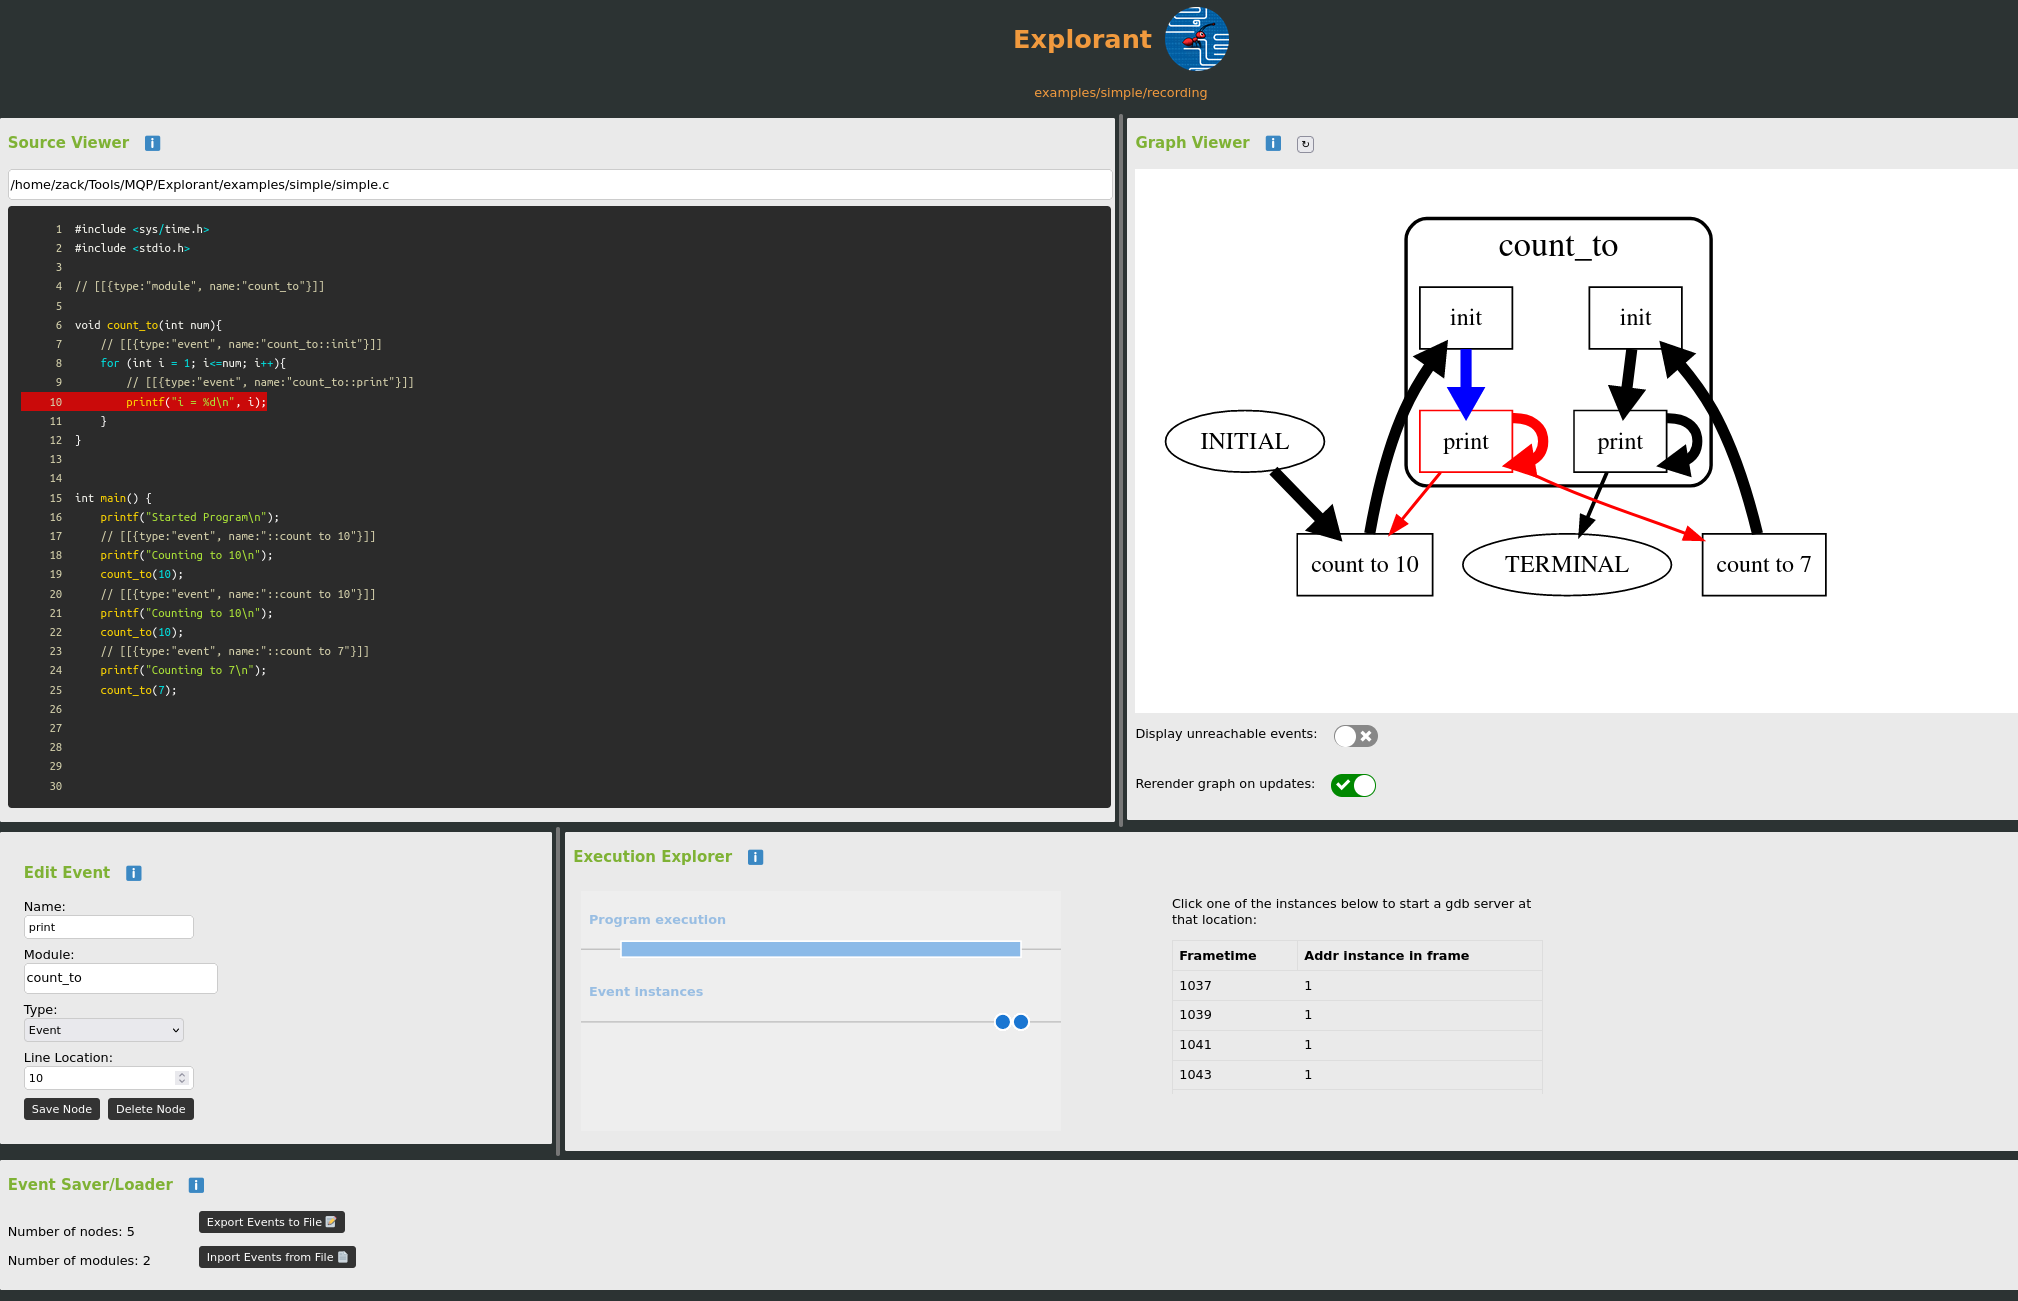
\includegraphics[scale=0.2]{design-whole}
    \caption{Image of the UI for Explorant}
    \label{fig:graph-whole}
\end{figure}

\subsection{Graph Viewer}
\begin{figure}[!ht]
    \centering
    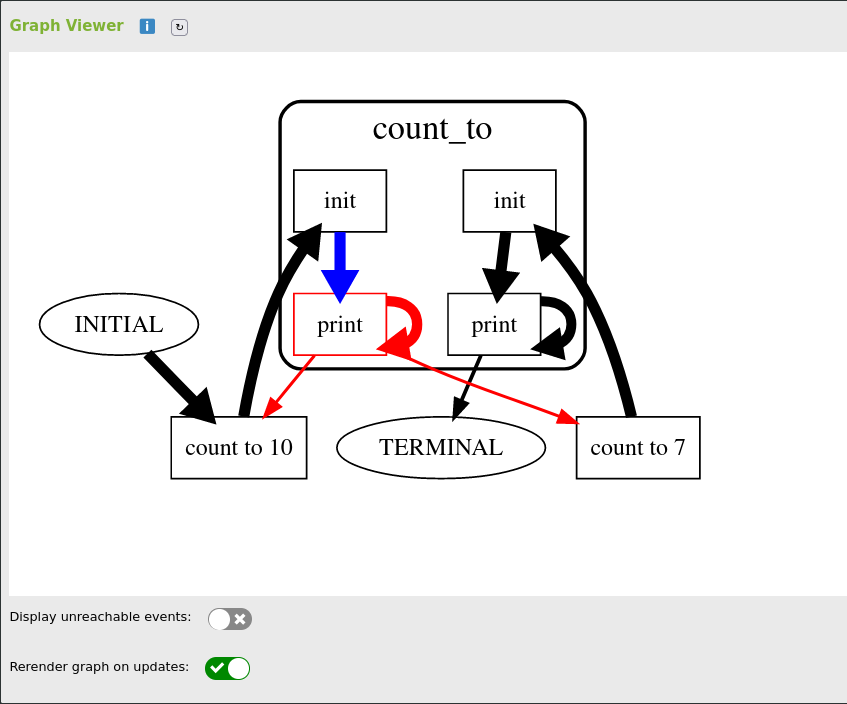
\includegraphics[scale=0.4]{design-graph}
    \caption{Image of the graph visualizer}
    \label{fig:graph}
\end{figure}
One of the most important components in Explorant is the graph viewer. The graph viewer describes the relationships between events across the entire execution of a trace. The graph viewer tries to convey as much information as possible. Some of the most important of these techniques are: 
\begin{itemize}
    \item The currently selected event is highlighted and all of its incoming and exiting nodes are colored. 
    \item The size of the edges are colored based on how probable that edge is to be traversed. 
    \item Events are grouped into modules (Described in section \ref{sec:modules})
    \item Unreachable (Un-run) events can be toggled to only show the happy path that was actually executed during the trace.
    \item Hovering over an event shows what function it was defined in
\end{itemize}
You can see examples of these techniques in figure \ref{fig:graph} including the highlighted node \texttt{print}, the module \texttt{count\_to}, the varying sized edges, and the toggled unreachable events. 






\section{Source Viewer}
\begin{figure}[!ht]
    \centering
    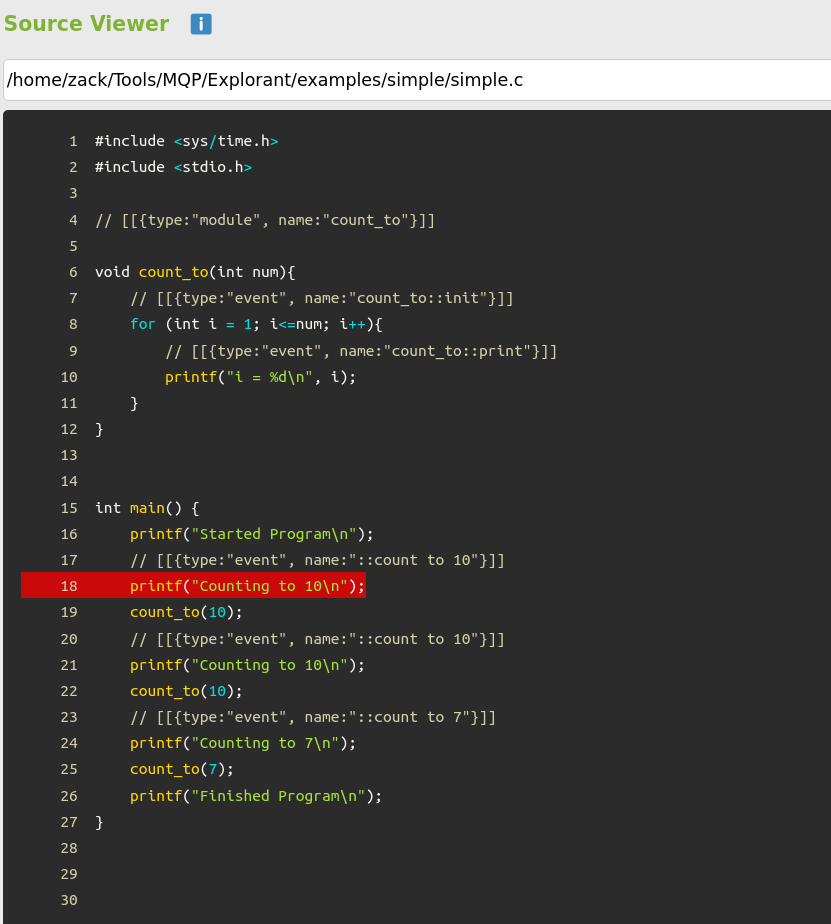
\includegraphics[scale=0.4]{design-source}
    \caption{Image of the source viewing component}
    \label{fig:graph-src}
\end{figure}
Another critical design criteria is that it must be easy for the developer to relate the high-level design to the source code easily. We addressed this by envisioning a simple source code viewer that contains features like syntax highlighting while also highlighting the line with the currently selected event in red. This allows developers to easily move back and forth between source code and the graph. The source viewer also can be right clicked to allow the developer to add new events to the graph in real time. You can see figure \ref{fig:graph-src} to see how this was implemented.


\section{Event Adding}
\begin{figure}[!ht]
    \centering
    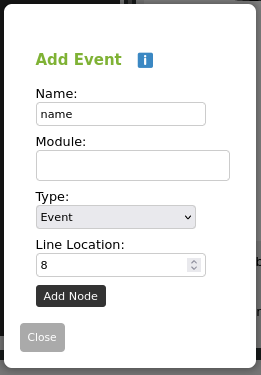
\includegraphics[scale=0.5]{design-adder}
    \caption{Image of the event adding component}
    \label{fig:graph-add}
\end{figure}
Our case study showed that it is critical that the developer is to be able to add new events after a trace has already been recorded. This ensures that the developer has a tight feedback loop that does not entail recompiling and rerunning a program every time they want to experiment and add to the graph. This component allows the user to define events, determine what module they reside in, and what line they pertain to. See figure \ref{fig:graph-add} to see how it was actually implemented. 


\section{Execution Explorer}
\begin{figure}[!ht]
    \centering
    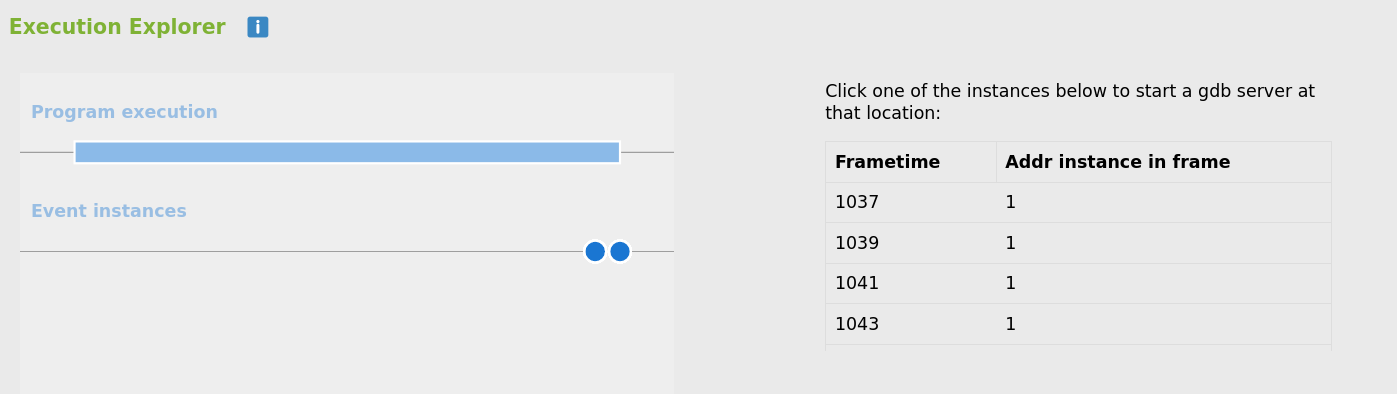
\includegraphics[scale=0.3]{design-explorer}
    \caption{Image of the execution explorer component}
    \label{fig:graph-exp}
\end{figure}
The last and perhaps most important constraint we considered when designing Explorant was the ability to dive deep when neccessary. A debugger like GDB is capable of providing the developer with the means to get a very close look at a particular moment in time. As such, we allow the developer to see a list of every time the event was reached, when it occured relative to the start of the program, and if they click on the particular instance of the event, it opens up gdb at that exact location. You can see figure \ref{fig:graph-exp} to see an image of how this was implemented. Note the timeline which shows all of the times the event was reached (with blue dots). The timeline also stacks some of these events because they occur so close together in time. 

\section{Design Limitations}
\label{sec:design-limitations}

\noindent This design has a few major limitations that are worth examining:

\begin{description}
    \item[JIT compilation / self modifying code] JITs \cite{jit} do not expose a standard method to access their location in the source code in the same way that static compilers provide DWARF data. This means that it is currently not feasible to instrument an arbitrary JIT compiler or code that it is running. Unfortuately, this means that many common languages like Java, Javascript, and Python will not work with Explorant.
\item[Macro heavy code] Macros hide a lot of information that DWARF data is unable to process as the macro is expanded in many locations and does not translate well. 
\item[Long running programs] Because we must run the whole trace every time we rebuild the graph (in case an address was executed in a spot we didn't expect), working with long running programs is difficult and painful. We could address this by either allowing the user to only analyze a certain time-range within the trace (which is equivalent to just ignoring the problem), or we could employ a much more advanced strategy where we instrument all function calls and then build heatmaps for where a new event could have been run and then only rerun those time segments. In either case, the current design and does not allow for efficient manipulation of long living programs. 
\item[Optimization levels] If a program is compiled with high optimization levels (like O3 in gcc \cite{gcc}) then functions can be inlined, loops can be unrolled, and the DWARF data becomes harder to parse, and every line is no longer guaranteed to have assembly instructions associated with it. As such, this design means that the user must be sure to compile the program without optimization. This is particularly important because some programs like glibc cannot be compiled without optimization (glibc requires at least O2), meaning that sometimes annotations inside of \begin{tt}malloc\end{tt} do not behave as we expect them to. 
\item[Browser dependent] The frontend is rendered in a browser. While this enables a fast development cycle, it also means that the final UI is much slower and heavier than a native app. 

\end{description}
